\section{DATA PREDICTIVE CONTROL}
\label{S:dpc}

The central idea behind DPC is to obtain control-oriented models using machine learning or black-box modeling, and formulate the control problem in a way that receding horizon control (RHC) can still be applied and the optimization problem can be solved efficiently.

Consider a black-box model given by $x_{k+1}=f(x_k,u_k,d_k)$, where $x,u,d$ represent states, inputs and disturbances, respectively. Depending upon the learning algorithm, $f$ is typically nonlinear, nonconvex and sometimes nondifferentiable (as is the case with regression trees and random forests) with no closed-form expression. 
Such functional representations learned through black-box modeling may not be directly suitable for control and optimization as the optimization problem can be computationally intractable, or due to nondifferentiabilities we may have to settle with a sub-optimal solution using evolutionary algorithms \cite{Kusiak2009}.
These problems can be eliminated by decomposing 
\begin{align}
f(x_k,u_k,d_k)= g(x_k,h(u_k),d_k),
\label{E:sepvars}
\end{align}
where both $g$ and $h$ are learned using the data, and $h(u_k)$ is convex and differentiable, and thus suitable for optimization. DPC uses this functional decomposition or \textit{separation of variables} to overcome the aforementioned challenges with black-box optimization.

%First, as the receding horizon involves predicting states into the future, with a black-box model trained on control variables as features, the optimization problem can be computationally intractable as the functions are typically nonlinear, nonconvex and do not have a closed-form expression.
%Second, black-box models like trees and random forests are not suitable for optimization because the gradient is not defined, so we may have to settle with a sub-optimal solution using evolutionary algorithms \cite{Kusiak2009}. 
%Third, interpretability is a desirable characteristic of a predictive model which only a few black-box models satisfy.
%DPC uses regression trees and tree ensembles (in particular random forests) for closed-loop RHC which overcome both the challenges by using \textit{separation of variables} which we explain next.
%Regression trees are interpretable by design. 
%The remaining problems are solved by using \textit{separation of variables} which we explain next.

\subsection{Separation of Variables}
\label{SS:sepvar}
%Consider a multivariable dynamical system subject to external disturbances. 
We distinguish between two sets of variables: control (or manipulated) variables $\tX^c \in \R^c$ and disturbance (or non-manipulated) variables $\tX^d \in \R^d$. The union of the two sets forms the full feature set for training, i.e. $\tX \equiv \tX^c \cup \tX^d \in \R^{c+d}$.
Our goal is to replace a model-based controller with a data-driven controller, where the latter depends only on the historical sensor data. 
These measurements could directly represent one or more states in the model-based control framework. We denote these as outputs $\tY \in \R$ for training, i.e. a $\tY$ represents a particular output and we can have separate models for multiple outputs. We define the number of training samples by $|(\tX,\tY)| = n$.

Using separation of variables, the training process is divided into two steps. \textit{Step 1:} The trees and the ensembles are trained only on $\tX^d$, which eases the computational complexity. It is important to note that besides external disturbances, $\tX^d$ also contains autoregressive terms of the output $\tY$ which is the main reason for the state space explosion. \textit{Step 2:} Linear regression models are trained in the leaves (or terminal nodes) of the trees which are function of only $\tX^c$. We have validated this linear model assumption in \cite{Jain2016}. As we shall see in Sec.~\ref{SS:dpcrt} and \ref{SS:dpcrf}, the second step reduces the run-time control problem into a convex program. This process is illustrated in Fig.~\ref{F:dpc-sepvars}.
\begin{figure}[t!]
	\centering
	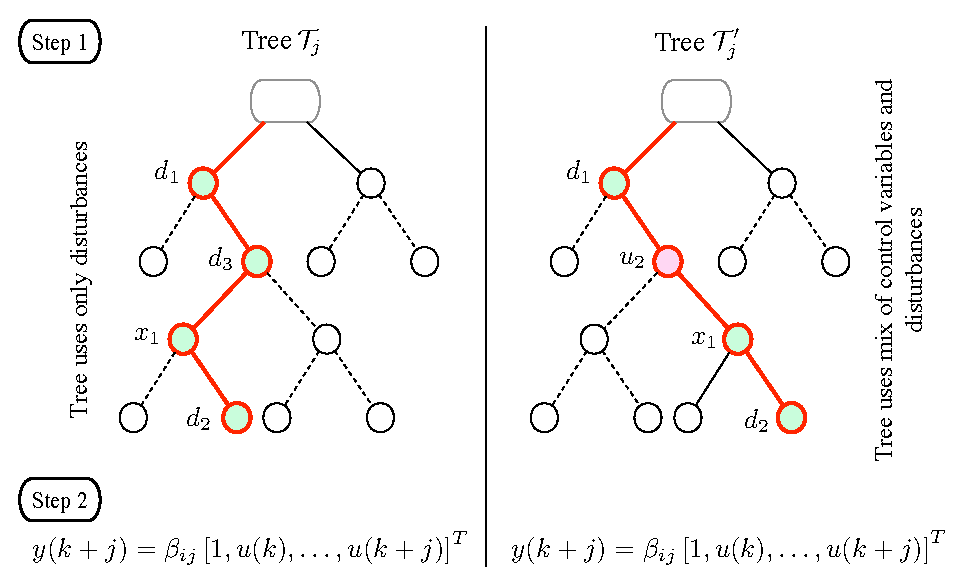
\includegraphics[width=20pc]{figures/dpc-sepvars.eps}
	\caption{Separation of variables. \textit{Step 1:} Tree $\mathcal{T}_1$ is trained only on the disturbances $\tX_d$ as the features. Tree $\mathcal{T}_2$ uses both the disturbances $\tX_d$ and the control variables $\tX_c$ for splitting and is thus not computationally suitable for control. \textit{Step 2:} In the leaf $R_i$ of the trees, a linear regression model parametrized by $\beta_i$ is defined as a function only of the control variables.}
	\captionsetup{justification=centering}
	\label{F:dpc-sepvars}
\end{figure}

\subsection{DPC-RT: DPC with Regression Trees}
\label{SS:dpcrt}
When the data has lots of features, which interact in complicated, nonlinear ways, assembling a single global model such as linear or polynomial regression can be difficult, and can lead to poor response predictions.
An approach to non-linear regression is to partition the data space into smaller regions, where the interactions are more manageable. 
This partition is repeated recursively until finally we get to small chunks of the data space where we can fit simple (eg. linear parametric) models. 
Therefore, in \eqref{E:sepvars}, the global model $f$ has two parts: the recursive partition $g$, and a linear (and convex) model $h$ for each cell of the partition.
%The algorithm for learning regression trees (CART) is described in~\cite{Breiman1984}.

Now, our goal is to predict the state $\tY$ at time $k$ for next $N$ time steps, i.e. $\tY_{\mathrm{k+1|k}},\dots,\tY_{\mathrm{k+N|k}}$, where $N$ is the control horizon. Applying the separation of variables, we build $N$ regression trees using CART procedure \cite{Breiman1984} such that the output $\tY_{\mathrm{k+j|k}}$ of the $j^{th}$ tree depends upon the previous $N$ disturbances:
\begin{gather}
\label{E:model_tree}
\tY_{\mathrm{k+j|k}} = \mathit{f}_{\mathrm{tree}} \left( \tX^d_{\mathrm{k+j-N|k}} ,\dots,\tX^d_{\mathrm{k+j-1|k}}  \right), \\ \nonumber
\mathsf{X}^d_{\mathrm{k+j-l|k}} \in \R^d \  \ \forall \ l,j=1,\dots,N.
\end{gather}
Then, the linear models as functions of $\tX^c$ in each leaf of the tree $\mathcal{T}_j$ are defined as
\begin{gather}
\label{E:model_leaf}
\tY_{\mathrm{k+j|k}} =  \beta^T_j [1,\tX^c_{\mathrm{k|k}},\dots,\tX^c_{\mathrm{k+j-1|k}} ]^T, \\ \nonumber
\mathsf{X}^c_{\mathrm{k+j-l|k}} \in \R^c \  \ \forall \ l,j=1,\dots,N.
\end{gather}
Note that the coefficients $\beta_j$ would be different for each leaf. Eq.~\eqref{E:model_leaf} implies that the prediction of output $\tY_{\mathrm{k+j}}$ at time $k$ is an affine combination of control inputs from time $k$ to $k+j-1$. Thus, we have managed to linearize the original model dynamics via black-box modeling. This two-step training is done offline. In run-time, given the disturbances $\tX^d_\mathrm{k|k}$ at time $k$, we can narrow down to a leaf of each tree in \eqref{E:model_tree} to retrieve the linear models in \eqref{E:model_leaf}.

In run-time, when a new control action is to be determined, each tree (prediction step) contributes to a linear constraint in the optimization as a replacement for the state dynamics in the case of MPC. Thus, the RHC optimization problem with a quadratic cost ($\mathcal{Q} \geq 0, \mathcal{R} \succeq 0$) can be formulated as:
\begin{align}
\begin{aligned}
\text{min } & \sum_{j=1}^{N} ({\tY}_{\mathrm{k+j|k}})^2 \mathcal{Q} + {\tX^c}^T_{\mathrm{k+j-1|k}} \mathcal{R} {\tX^c}_{\mathrm{k+j-1|k}} +  \lambda\epsilon_j\\
\text{s.~t. } & \ \ \ \ \ \tY_{\mathrm{k+j|k}} =  \beta^T [1,\tX^c_{\mathrm{k|k}},\dots,\tX^c_{\mathrm{k+j-1|k}} ]^T \\
& \ \ \ \ \ \ \ \ \ \ \ \ \ \ \ \underline{\tX}^c \leq \tX^c_{\mathrm{k+j-1|k}} \leq \bar{\tX}^c\\ 
& \ \ \ \ \ \ \ \ \ \ \ \ \underline{\tY}-\epsilon_j \leq \tY_{\mathrm{k+j|k}} \leq \bar{\tY} + \epsilon_j\\\
& \ \ \ \ \ \ \ \ \ \ \ \ \ \ \epsilon_j \geq 0, \ j = 1,\dots,N.
\end{aligned}
\label{E:dpcrt}
\end{align}
Here, $\mathcal{Q} \in \mathbb{R}$ and $\mathcal{R} \in \mathbb{R}^{c \times c}$, and the slack variables $\epsilon_j$ ensure recursive feasibility since the equality constraint on $\tY$ is relaxed. Of course, a different cost function can be chosen depending upon the application. In the current formulation, the data-driven control problem is reduced to a convex program which is much easier to solve than running an optimization directly on a black-box model trained on $\tX^c$ as features. We solve this optimization in the same manner as MPC to determine the optimal sequence of inputs $[\tX^c_{\mathrm{k|k}},\dots,\tX^c_{\mathrm{k+N-1|k}}]$, apply the first control input $\tX^c_{\mathrm{k|k}}$ and proceed to the next time step $k+1$. The pseudo code for DPC-RT is given in Alg.~\ref{A:dpcrt}.

\subsection{DPC-En: DPC with Ensemble Methods}
\label{SS:dpcrf}
Regression trees obtain good predictive accuracy in many domains. However, the models used in their leaves have some limitations regarding the kind of functions they are able to approximate.
The problem with trees is their high variance and that they can overfit the data easily.
A small change $\delta$ in the data can result in a different series of splits and thus violate the acceptable accuracy $\eps$.
This is the price to be paid for estimating a tree-based structure from the data.
%The main reason behind this is the hierarchical nature of the process: the effect of an error in the top split is propagated down to all of the splits below it.
%While pruning and cross validation can help reduce the over fitting partially, we use ensemble methods for growing more accurate trees.

We use ensemble methods \cite{Friedman2001} to combine the predictions of several independent regression trees in order to improve generalizability and robustness over a single estimator. 
%Random forests or \textit{tree-bagging} are a type of ensemble method which makes predictions by averaging over the predictions of several independent trees.
The essential idea is to average many noisy trees to reduce the overall variance in prediction.
We inject randomness into the tree construction in two ways. First, we randomize the features used to define splitting in each tree.
Second, we build each tree using a bootstrapped or sub-sampled data set.
In this way, each tree in the forest is trained on different data, which introduces differences between the trees. More explicitly, training features $\tX^d \in \R^p$ with $p<d$ and the in-bag samples (in-bag samples correspond to the data samples on which the tree was trained) are different for each tree in the forest i.e $|(\tX,\tY)|<n$.

The goal with DPC-En is to replace each tree in Alg.~\ref{A:dpcrt} by a forest
\begin{gather}
\label{E:model_forest}
\tY_{\mathrm{k+j|k}} = \mathit{f}_{\mathrm{forest}} \left( \tX^d_{\mathrm{k+j-N|k}} ,\dots,\tX^d_{\mathrm{k+j-1|k}}  \right), \\ \nonumber
\mathsf{X}^d_{\mathrm{k+j-l|k}} \in \R^p \  \ \forall \ l,j=1,\dots,N,
\end{gather}
which, again, is trained only on $\mathsf{X}^d$, with $\tX^d \in \R^p \subset \R^d$ for each tree,  and then fit a linear regression model using $\mathsf{X}^c$ in every leaf of every tree. We build $N$ such forests for $N$ prediction steps such that the leaf $R_i$ of forest $\mathcal{R}_j$ uses a linear model
\begin{gather}
\label{E:model_leaf_forest}
\tY_{\mathrm{k+j|k}} =  \Theta^T_{ij} [1,\tX^c_{\mathrm{k|k}},\dots,\tX^c_{\mathrm{k+j-1|k}} ]^T, \\ \nonumber
\mathsf{X}^c_{\mathrm{k+j-l|k}} \in \R^c \  \ \forall \ l,j=1,\dots,N.
\end{gather}
Here $(\mathsf{X}^c,\mathsf{Y})$ correspond to the in-bag samples for the trees.

\begin{algorithm}[t!]
	\caption{Data Predictive Control with Regression Trees}
	\label{A:dpcrt}
	\begin{algorithmic}[1]
		\State \textsc{Design Time}
		\Procedure{Model Training using Separation of Vars}{}
		\State Set $\mathsf{X}^c$ $\gets$ manipulated features
		\State Set $\mathsf{X}^d$ $\gets$ non-manipulated features
		\State Build $N$ predictive trees with $(\tY,\tX^d)$ defined in \eqref{E:model_tree}
		\ForAll{trees $\mathcal{T}_j$}
		\ForAll{regions $R_i$ at the leaves of $\mathcal{T}_j$}
		\State Fit $ \tY_{\mathrm{k+j|k}} =  \beta^T_j \left[1,\tX^c_{\mathrm{k|k}},\dots,\tX^c_{\mathrm{k+j-1|k}} \right]^T$ as in \eqref{E:model_leaf}
		\EndFor
		\EndFor
		\EndProcedure
		\State \textsc{Run Time}
		\Procedure{Predictive Control}{}
		\While{$k< k_{\mathrm{stop}}$}
		\ForAll{trees $\mathcal{T}_j$}
		\State Determine the leaf $R_i$ using $\tX^d$ as in \eqref{E:model_tree}
		\State Obtain the linear model at $R_{i}$ trained in \eqref{E:model_leaf}
		\EndFor
		\State Solve optimization in \eqref{E:dpcrt} to determine optimal
		\State control actions $[\tX^c_{\mathrm{k|k}},\dots,\tX^c_{\mathrm{k+N-1|k}}]$
		\State Apply the first input $\tX^c_{\mathrm{k|k}}$
		\EndWhile
		\EndProcedure
	\end{algorithmic}
\end{algorithm}

While the offline training burden in DPC-En is slightly increased compared to DPC-RT, in the control step we exploit the better accuracy, and lower variance properties of the random forest. 
If a forest has $t$ number of trees, given the forecast of disturbances, we have $t$ sets of linear coefficients. We simply average out all the coefficients from all the trees to get one linear model represented by $\hat{\Theta}_j$ for each forest. Note that the averaging step can only be done in run-time because the leaf of each tree can be narrowed down only when the $\tX^d$ is known. Thus, for $N$ forests, we again have exactly $N$ linear equality constraints in the optimization problem below:
\begin{align}
\begin{aligned}
\text{min } & \sum_{j=1}^{N} ({\tY}_{\mathrm{k+j|k}})^2 \mathcal{Q} + {\tX^c}^T_{\mathrm{k+j-1|k}} \mathcal{R} {\tX^c}_{\mathrm{k+j-1|k}} +  \lambda\epsilon_j\\
\text{s.~t. } & \ \ \ \ \ \tY_{\mathrm{k+j|k}} =  \hat{\Theta}^T_j [1,\tX^c_{\mathrm{k|k}},\dots,\tX^c_{\mathrm{k+j-1|k}} ]^T \\
& \ \ \ \ \ \ \ \ \ \ \ \ \ \ \ \underline{\tX}^c \leq \tX^c_{\mathrm{k+j-1|k}} \leq \bar{\tX}^c\\ 
& \ \ \ \ \ \ \ \ \ \ \ \ \underline{\tY}-\epsilon_j \leq \tY_{\mathrm{k+j|k}} \leq \bar{\tY} + \epsilon_j\\\
& \ \ \ \ \ \ \ \ \ \ \ \ \ \ \epsilon_j \geq 0, \ j = 1,\dots,N.
\end{aligned}
\label{E:dpcrf}
\end{align}
DPC-En is graphically described in Fig.~\ref{F:dpc-algo-rf}. The ensemble data predictive control (DPC-En) is the first such method to bridge the gap between ensemble predictive models (such as random forests) and receding horizon control. In the next section, we compare DPC-RT and DPC-En to MPC for a building model.